% Created 2021-07-21 Mi 17:58
% Intended LaTeX compiler: pdflatex
\documentclass[bigger]{beamer}
\usepackage[utf8]{inputenc}
\usepackage[T1]{fontenc}
\usepackage{graphicx}
\usepackage{grffile}
\usepackage{longtable}
\usepackage{wrapfig}
\usepackage{rotating}
\usepackage[normalem]{ulem}
\usepackage{amsmath}
\usepackage{textcomp}
\usepackage{amssymb}
\usepackage{capt-of}
\usepackage{hyperref}
\mode<beamer>{\useinnertheme{rounded}\usecolortheme{rose}\usecolortheme{dolphin}\setbeamertemplate{navigation symbols}{}\setbeamertemplate{footline}[frame number]{}}
\mode<beamer>{\usepackage{amsmath}\usepackage{ae,aecompl,sgamevar,tikz}}
\let\oldframe\frame\renewcommand\frame[1][allowframebreaks]{\oldframe[#1]}
\setbeamertemplate{frametitle continuation}[from second]
\newcommand{\Ra}{\Rightarrow} \newcommand{\ra}{\rightarrow} \newcommand{\Lra}{\Leftrightarrow}
\usetheme{default}
\author{Christoph Schottmüller}
\date{}
\title{Bayes Nash equilibrium}
\hypersetup{
 pdfauthor={Christoph Schottmüller},
 pdftitle={Bayes Nash equilibrium},
 pdfkeywords={},
 pdfsubject={},
 pdfcreator={Emacs 27.2 (Org mode 9.4.4)}, 
 pdflang={English}}
\begin{document}

\maketitle

\begin{frame}[label={sec:org6c62038}]{Introduction}
\begin{itemize}
\item so far
\begin{itemize}
\item need to look at games of incomplete information (preference aggregation when preferences are private, auctions)
\item under certain assumptions decision makers can be modeled as expected utility maximizers
\end{itemize}
\item still missing
\begin{itemize}
\item how to react to information?
\item strategic interaction under uncertainty
\end{itemize}
\end{itemize}
\end{frame}


\section{Bayes' rule}
\label{sec:org28df2d3}
\begin{frame}[label={sec:orgc8ba334}]{Bayes' rule: A simple example}
\begin{itemize}
\item I know someone who lives in Munich. What is the probability that this person is male?
\item I know someone who lives in Munich and who is 1.90 m tall. What is the probability that this person is male?
\item I know someone who lives in Munich and has green eyes. What is the probability that this person is male?
\end{itemize}
\end{frame}
\begin{frame}[label={sec:org8165c6a}]{Bayes' rule}
\begin{block}{Bayes' rule}
For two events \(A\) and \(B\)
$$P(A|B)=\frac{P(B|A) P(A)}{P(B)}.$$
\end{block}

\begin{itemize}
\item easier to remember as \(P(A|B)P(B)=P(B|A)P(A)\) which is also equal to \(P(A\cap B)\)
\item hence, \(P(A|B)=P(A\cap B)/P(B)\)
\end{itemize}

\begin{figure}   
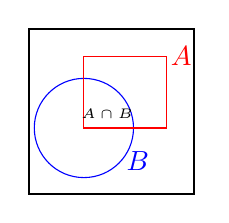
\begin{tikzpicture}[scale=0.7]
\draw[thick] (0,0) rectangle (3,3) ;
\draw [blue] (1,1.2) circle [radius=0.9];
\draw[red] (1,1.2) rectangle (2.5,2.5) ;
 \node[right,red] at (2.4,2.5) {$A$};
\node[right,blue] at (1.6,0.6) {$B$};
\node at (1.42,1.45) {\tiny$A\cap B$}; 
\end{tikzpicture}
\end{figure}
\end{frame}

\begin{frame}[label={sec:orgcfbb15d}]{Bayes' rule: example}
\begin{itemize}
\item an antigen test for a certain virus is 70\% reliable at detecting an illness and 99.5\% reliable at correctly reporting that somebody is healthy
\item suppose about 80.000 people are currently infected with the virus
\item suppose 80 million people live in Germany
\item if a random person is takes a test and the test is positive, what is the probability that this person is infected?
\end{itemize}
\end{frame}
\begin{frame}[label={sec:org8d2acd6}]{Bayes' rule: comments}
\begin{itemize}
\item calculations are reasonably simple
\item intuition often goes wrong when the prior is extremely skewed
\item make sure to understand it as it will often loom in the background
\end{itemize}
\end{frame}
\begin{frame}[label={sec:org2e23cd4}]{Independence}
\begin{block}{Independence}
Two random variables \(X\) and \(Y\) are independent if
 $$P(X=x,Y=y)=P(X=x)P(Y=y).$$
\end{block}

\begin{itemize}
\item by Bayes' rule, \(P(X=x|Y=y)=P(X=x)\) if \(X\) and \(Y\) are independent
\begin{itemize}
\item knowing \(Y\) does not affect my belief about \(X\)
\end{itemize}

\item independence will often be assumed to keep the models simple
\end{itemize}
\end{frame}
\section{Games of incomplete information}
\label{sec:org2658cef}
\begin{frame}[label={sec:org8b5aa18}]{Games of incomplete information I: an example}
\begin{itemize}
\item an incumbent decides whether to build a new plant (I for invest)  at cost \(c\)
\item entrant simultaneously decides whether to enter (E)
\item entrant does not know whether \(c\) is "low" (\emph{l}) or "high" (\emph{h})
\end{itemize}

\begin{table}[htbp]
\caption{Payoffs with \(c=h\)}
\centering
\begin{tabular}{l|ll}
 & E & NE\\
\hline
I & 0,-1 & 2,0\\
NI & 2,1 & 3,0\\
\end{tabular}
\end{table}
\begin{table}[htbp]
\caption{Payoffs with \(c=l\)}
\centering
\begin{tabular}{l|ll}
 & E & NE\\
\hline
I & 1.5,-1 & 3.5,0\\
NI & 2,1 & 3,0\\
\end{tabular}
\end{table}

\begin{itemize}
\item how to solve this game?
\end{itemize}
\end{frame}

\begin{frame}[label={sec:orga91b360}]{Games of incomplete information II: an example}
\begin{itemize}
\item entrant has to think about
\begin{itemize}
\item how likely is it that incumbent has low cost or high cost?
\item what will incumbent do if he has high cost? what if he has low cost?
\item what should I do?
\end{itemize}

\item incumbent with low cost has to think about
\begin{itemize}
\item what will entrant do?
\begin{itemize}
\item partly depends on what he thinks I would do if I had high costs\ldots{}
\end{itemize}
\end{itemize}

\item we will return to this example later on!
\end{itemize}
\end{frame}
\begin{frame}[label={sec:org00ce779}]{Games of incomplete information III: general thoughts}
\begin{itemize}
\item say two firms do not know the cost of the respective other firm
\item the main trick:
\begin{itemize}
\item add beliefs about costs of other firm (i.e. a probability distribution over possible costs)
\item maximize expected utility
\end{itemize}
\item we might want to allow this belief to depend on own costs
\begin{itemize}
\item e.g. a high cost firm may think it is more likely that the other firm has also high costs
\end{itemize}
\end{itemize}
\end{frame}

\begin{frame}[label={sec:orgfa73986}]{Games of incomplete information IV: formal description}
\begin{itemize}
\item finite set of players: \(i=1,\dots,N\)
\item each player has a set of pure strategies \(S_i\)
\item to capture uncertainty of other players:
\begin{itemize}
\item player \(i\) has a \alert{type} \(t_i\) from a set \(T_i\)
\item player \(i\) knows his own type \(t_i\) but other players do not
\end{itemize}
\item player \(i\) maximizes expected utility with Bernoulli utility function \(u_i:S\times T\ra\Re\)
\begin{itemize}
\item \(T=\times_{i=1}^N T_i\) is set of all type profiles
\item \(S=\times_{i=1}^N S_i\) is set of all strategy profiles
\item actions and types of all players can affect \(i\)'s payoff
\end{itemize}
\item each type of each player has a belief \(p_i(t_{-i}|t_i)\) about other players' types
\begin{itemize}
\item \(p_i(t_{-i}|t_i)\in[0,1]\)
\item \(\sum_{t_{-i}\in T_{-i}}p_i(t_{-i}|t_i)=1\) where \(T_{-i}\) is the set of type profiles of all players but \(i\)
\end{itemize}
\end{itemize}
\end{frame}
\begin{frame}[label={sec:orgdc87d62}]{Games of incomplete information V:  formal description (short)}
A \emph{N}-player game of incomplete information can be denoted as \(G=(S_i,T_i,p_i,u_i)_{i=1}^N\) where
\begin{itemize}
\item \(S_i\) is the strategy set of player \(i\)
\item \(T_i\) is the type set of player \(i\)
\item \(p_i\) assigns to each \(t_i\in T_i\) a belief over \(T_{-i}\)
\item \(u_i:S\times T\ra\Re\) is player \(i\)'s utility function.
\end{itemize}
If all \(S_i\) and \(T_i\) are finite, the \(G\) is called a \emph{finite game of incomplete information.}     
\end{frame}

\begin{frame}[label={sec:org6bf1273}]{Games of incomplete information VI: assumptions on beliefs}
\begin{itemize}
\item usually, it is assumed that types have a joint distribution \(p\) (over \(T\)) and beliefs are derived using Bayes' rule:
$$p_i(t_{-i}|t_i)=\frac{p(t_i,t_{-i})}{\sum_{t_{-i}'\in T_{-i}}p(t_i,t_{-i}')}$$
then \(p\) is called the \emph{common prior}
\item often we assume independence of types, i.e. the belief \(p_i(t_{-i}|t_i)\) is the same for all \(t_i\)
\end{itemize}
\end{frame}
\section{Bayesian Nash equilibrium}
\label{sec:org32bb812}

\begin{frame}[label={sec:org04c1035}]{Bayesian Nash equilibrium I}
each player maximizes expected utility given his type and others strategies\linebreak
\(\ra\) trick:
\begin{itemize}
\item think of each type of every type as an own player maximizing expected utility (with utility function \(u_i\) and beliefs \(p_i(t_{-i}|t_i)\))
\item a Bayesian Nash equilibrium consists of one strategy for each type of each player such that
\begin{itemize}
\item the strategy of type \(t_i\) maximizes expected utility of player \(i\) given the strategies of the others and the belief \(p_i(\cdot|t_i)\)
\end{itemize}
\end{itemize}
\end{frame}

\begin{frame}[label={sec:orgc37b21e}]{Bayesian Nash equilibrium II (formal)}
For Bayesian game \(G=(S_i,T_i,p_i,u_i)_{i=1}^N\), define the auxiliary game of complete information \(G'\):
\begin{itemize}
\item set of players is \(T_1\cup T_2\cup \dots\cup T_N\)
\item strategy set of player \(t_i\) is \(S_i\)
\item von Neumann-Morgenstern utility \(v_{t_i}(s)=\mathbb{E}_{t_{-i}\in T_{-i}}[u_i(s(t_1),\dots,s(t_N),t,\dots,t_N)]\)
\begin{itemize}
\item where \(s(t_i)\) is the strategy of player \(t_i\) and \(s=(s(t_1),\dots,s(t_N))\)
\item where expectation is take using the belief \(p_i(\cdot|t_i)\)
\end{itemize}
\end{itemize}

\begin{block}{Definition: Bayesian Nash equilibrium (BNE)}
A (mixed) Bayesian Nash equilibrium of game \(G\) is a (mixed) Nash equilibrium of the corresponding auxiliary game \(G'\).
\end{block}
\end{frame}

\begin{frame}[label={sec:org048c702}]{Bayesian Nash equilibrium III: back to example}
\begin{itemize}
\item assume the belief \(p_E(l)=p_E(h)=1/2\)
\end{itemize}

\begin{table}[htbp]
\caption{Payoffs with \(c=h\)}
\centering
\begin{tabular}{l|ll}
 & E & NE\\
\hline
I & 0,-1 & 2,0\\
NI & 2,1 & 3,0\\
\end{tabular}
\end{table}
\begin{table}[htbp]
\caption{Payoffs with \(c=l\)}
\centering
\begin{tabular}{l|ll}
 & E & NE\\
\hline
I & 1.5,-1 & 3.5,0\\
NI & 2,1 & 3,0\\
\end{tabular}
\end{table}

\begin{itemize}
\item what is the optimal strategy for type \(h\)?
\item if type \(l\) invests with probability \(s(l)\), what is the entrant's best response?
\item if the entrant enters with probability \(s(e)\), what is type \(l\)'s best response?
\end{itemize}
\end{frame}

\begin{frame}[label={sec:orgf065b30}]{public good example I}
\begin{itemize}
\item \(N\) guests at a garden party
\item each guest has to decide whether to bring a speaker to play music, \(S_i=\{0,1\}\)
\item payoff of player \(i\):
\begin{itemize}
\item zero if no one brings a speaker
\item \(t_i\) if someone else brought a speaker
\item \(t_i-1/2\) if person \(i\) brought a speaker
\end{itemize}
\item \(t_i\) are independently distributed and \(1\) (high) with probability \(2/3\) and \(0\) (low) with probability \(1/3\)
\item we want to find a \emph{symmetric BNE}, i.e. one where all high types use one strategy and all low types use one other strategy
\end{itemize}
\end{frame}

\begin{frame}[label={sec:orgfb6a1f7}]{public good example II}
\begin{itemize}
\item what is the optimal strategy of a low type?
\item suppose all high types bring a speaker with probability \(\alpha\)
\begin{itemize}
\item for player \(i\): what is the probability that no one else brings a speaker?
\end{itemize}

\begin{itemize}
\item what is the expected payoff for a high type of player \(i\) when bringing the speaker?
\end{itemize}

\begin{itemize}
\item what is the expected payoff for a high type of player \(i\) when not bringing the speaker?
\end{itemize}
\item which value of \(\alpha\) gives a BNE?

\vspace*{0.5cm}
\end{itemize}
\begin{figure}   
    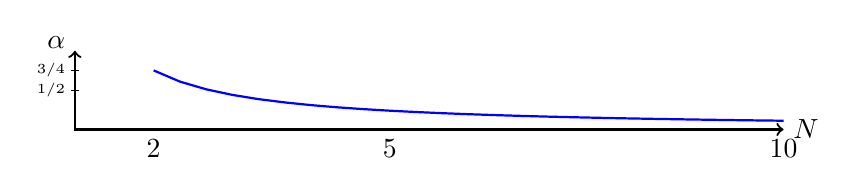
\begin{tikzpicture}
    \draw[<->,thick] (1,1) -- (1,0) -- (10,0);
    \draw[thick,domain=2:10, blue] plot (\x,{1.5*(1-(0.5)^(1/(\x-1)))});
    \node[left] at (1,1.1) {$\alpha$};
    \node[right] at (10,0) {$N$};
    \node[below] at (5,0){5};
    \node[below] at (2,0){2};
  \node[below] at (10,0){10};
  \node[left] at (1,0.5){\tiny 1/2};
   \draw (0.95,0.5)--(1.05,0.5);
   \draw (0.95,0.75)--(1.05,0.75);
\node[left] at (1,0.75){\tiny 3/4};
    \end{tikzpicture}
    \end{figure}
\end{frame}
\end{document}